\documentclass[10pt,journal,compsoc]{IEEEtran}
    \usepackage{caption}
    \usepackage{subcaption,array}
    \usepackage[pdftex]{graphicx}
    \usepackage{cite}
    \hyphenation{op-tical net-works semi-conduc-tor}
    
    
    \begin{document}
    
    \title{Mobile Robot's Position and Orientation using Adaptive Monte Carlo Localization}
    
    \author{Trim Bresilla}
    
    \markboth{Localization project, Robotics Nanodegree Program, Udacity}%
    {}
    \IEEEtitleabstractindextext{%
    
    \begin{abstract}
    This work describes one of the challenges in localization of mobile robotic. Using different probabilistic techniques and algorithms served by Robotic Operating System, by filtering noisy sensor data, we are able to get precise pose of mobile robot. To do that, we use a package - AMCL - that goes through sensor readings and estimates the pose and orientation of the mobile robot. Movebase, another ROS package takes those readings and uses for navigation stack, that the robot reaches the destination. While all this is run through the Gazebo simulator with its own physics engine (that utilizes collision, visuals etc...). By tunning AMCL's parameters we can estimate very accurately robot's pose and orientation and then navigate to goal position without any collision.
    \end{abstract}
    
    % Note that keywords are not normally used for peerreview papers.
    \begin{IEEEkeywords}
    Robot, IEEEtran, Udacity, \LaTeX, Localization.
    \end{IEEEkeywords}}
    
    
    \maketitle
    \IEEEdisplaynontitleabstractindextext
    \IEEEpeerreviewmaketitle
    \section{Introduction}
    \label{sec:introduction}
    
    \IEEEPARstart{L}{ocalisation} is one of the biggest challenge in mobile robotic. Determining robot's pose in mapped environment is very important for later activities like path-planning, manipulation etc. This is highly important in environment where precision very high (manufacturing). Using different probabilistic algorithms to filter noise from sensors (IMU, Rotary Encoders, Range-filters or 3D cameras). Filtering noisy signals is essential since many sensors have an output that is to noisy too be used directly, and different filter techniques lets you account for the uncertainty in the signal/state. One important use of generating non-observable states is for estimating velocity. It is common to have position sensors (encoders) on different joints; however, simply differentiating the position to get velocity produces noisy results. Navigation is one of the most challenging competencies required of a mobile robot. Success
    in navigation requires success at the four building blocks of navigation: perception - the robot must interpret its sensors to extract meaningful data; localization - the robot must determine its position in the environment; cognition - the robot must decide how to act to achieve its goals; and motion control -  the robot must modulate its motor outputs to achieve the desired trajectory.

    \section{Background}
    The general localization problem is composed by two increasingly difficult sub-problems. In the position tracking problem the robot knows its initial location in the environment. The goal of the localization is to keep track of the position while the robot is navigating through the environment. Methods that address this problem are called local techniques. In the global localization, instead, problem the robot does not know its initial position and it has to localize itself from scratch. It hereby possibly needs to be able to deal with multiple hypotheses about its location. Methods that solve this problem are called global techniques. An even harder problem is the kidnapped robot problem. The robot is already correctly localized but it is transferred (or “kidnapped”), to another location without the robot being aware of this. This can happen for example in the case of failures or if the robot is physically moved by an operator. The problem for the robot is to detect that it has been kidnapped and to find out what its new location is. In determining its location, a robot has access to two kinds of information. First, it has a-priori information gathered by the robot itself or supplied by an external source in an initialization phase. Second, the robot gets information about the environment through every observation and action it makes during navigation. In general, the a prior information supplied to the robot describes the environment where the robot is driving around. It specifies certain features that are time-invariant and thus can
    be used to determine a location.  As one of the fundamental problems in mobile robot navigation, many solutions (algorithms) are used to tackle this problem including approaches employing Kalman filtering, grid-based Markov localization,  or Monte Carlo methods.

    \begin{figure}[thptb]
        \centering
        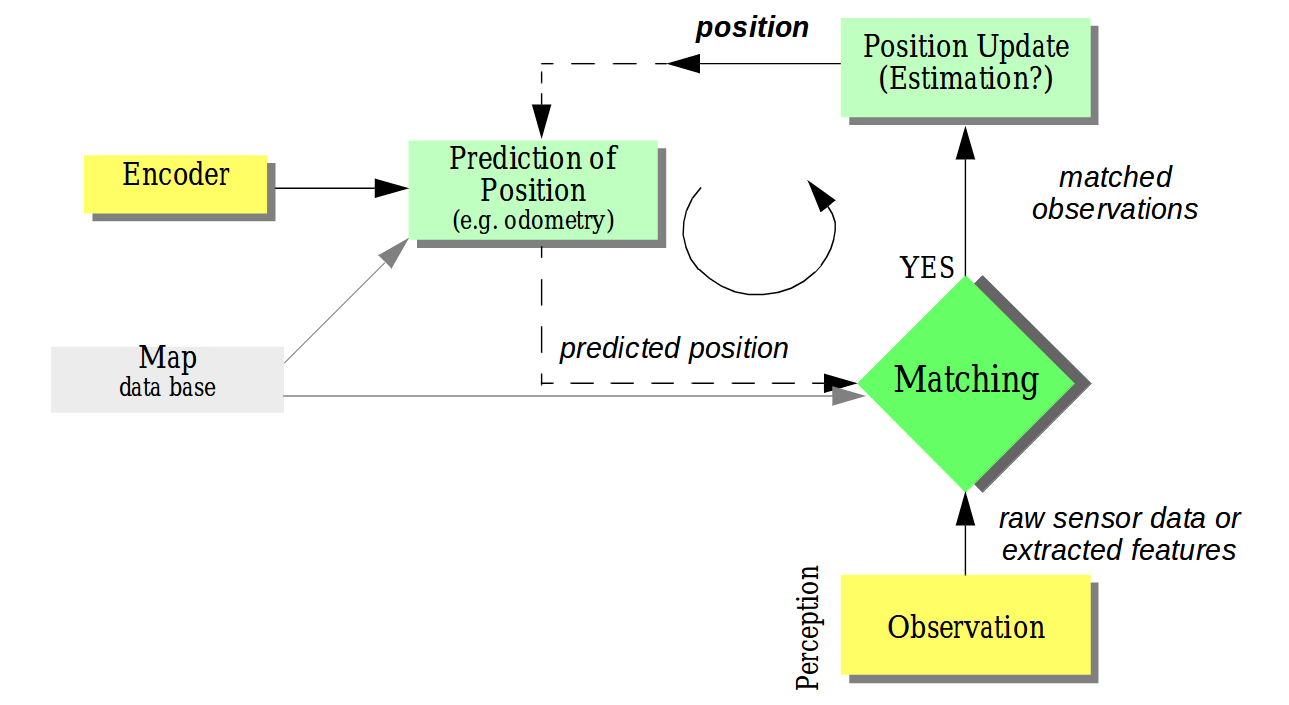
\includegraphics[width=\linewidth]{generalnav.png}
        \caption{General schematic for mobile robot localization}
        \label{fig:robot1}
    \end{figure}


    

    \subsection{Kalman Filters}
    The Extended Kalman Filter (EKF) has been used for many years to estimate the state of a nonlinear system from noisy measurements.It iss based on the linearization of the nonlinear maps around the estimated trajectory, and on the assumption that the initial state and measurement noises are Gaussian and uncorrelated each other. Basically uses a series of measurements observed over time, containing statistical noise and other inaccuracies, and produces estimates of unknown variables that tend to be more accurate than those based on a single measurement alone, by estimating a joint probability distribution over the variables for each timeframe.

    \subsection{Particle Filters}
    Adaptive Monte Carlo localization (AMCL), also known as particle filter localization, is an algorithm for robots to localize using a particle filter. Given a map of the environment, the algorithm estimates the position and orientation of a robot as it moves and senses the environment. The algorithm uses a particle filter to represent the distribution of likely states, with each particle representing a possible state, i.e., a hypothesis of where the robot is. The algorithm typically starts with a uniform random distribution of particles over the configuration space, meaning the robot has no information about where it is and assumes it is equally likely to be at any point in space. Whenever the robot moves, it shifts the particles to predict its new state after the movement. Whenever the robot senses something, the particles are resampled based on recursive Bayesian estimation, i.e., how well the actual sensed data correlate with the predicted state. Ultimately, the particles should converge towards the actual position of the robot.


    \begin{figure}[thptb]
        \centering
        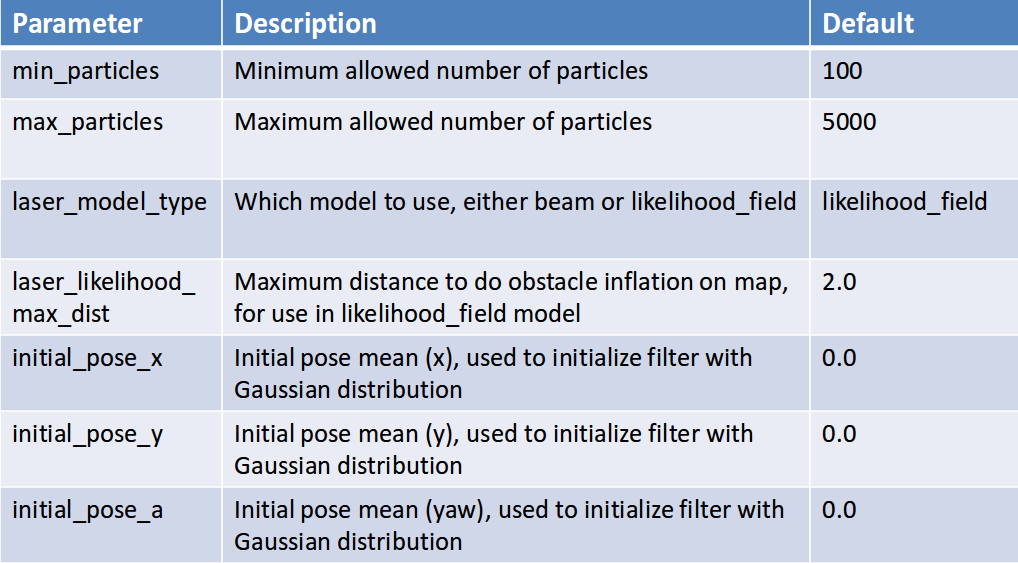
\includegraphics[width=\linewidth]{amcl.png}
        \caption{AMCL parameters}
        \label{fig:robot3}
    \end{figure}
    
    \subsection{Comparison / Contrast}
    Compared to all other algorithhs for localisation, AMCL by using sampling-based representation, has has
    several key advantages over earlier work in the field:
    \begin{enumerate}
        \item In contrast to existing Kalman filtering based techniques, it is able to represent multi-modal distributions and thus can globally localize a robot.
        \item It  drastically  reduces  the  amount  of  memory  required compared to grid-based localization and can integrate measurements at a considerably higher frequency.
        \item Can be easily controlled to focus resources to a more relevant area or interest points by sampling in proportion to the posterior likelihood.
        \item It is more accurate than Markov localization with a fixed cell size, as the state represented in  the samples is not discretized.
        \item By controlling the number of samples on-line, particle filters can adapt to the available computational resources.
        \item It is much easier to implement.
    \end {enumerate}

    \section{Simulations}
    The 3D simulation is performed with Gazebo , a 3D robot simulator. Gazebo is a complete physical simulation of robots including shapes, joints, contacts, collisions, and friction. Gazebo utilized the 3D framework for rendering the environment and objects.  It uses a physics engine that can simulate rigid body  dynamics. During the simulation, Gazebo publishes the models’ states and behaviors via the ROS middleware’s communication infrastructure so that all other nodes can use these parameters for triggering certain actions. Gazebo  uses  URDF  (Unified  Robot  Description  Format) files for the description of the models. The physical elements for the simulation can be modeled with all common 3D modeling tools such as Blender. Gazebo further offers the possibility to draw defined simple geometric objects, such as boxes, spheres, and cylinders  with  a  single  XML  tag.   All  of  these  simple  elements  or  meshed  elements,  i.e.  more complex  polyhedral objects, can be linked together with joints. Gazebo distinguishes between different kinds of joints to be able to calculate their physical state. This enables to confine the degrees of freedom to the desired ones. By defining a mass, inertia and friction values for an element, the physics engine can simulate its dynamic behavior in a realistic way.

    In our case, we simulate a differential wheel robot. This is the most common control mechanism for robot builders, especially for beginners. The concept is simple; Velocity difference between two motors drive the robot in any required path and direction. Hence the name “Differential” drive. Differential wheeled robot can have two independently driven wheels fixed on a common horizontal axis or three wheels where two independently driven wheels and a roller ball or a castor attached to maintain equilibrium. Controlling a differential robot can be difficult sometimes. Since the drive wheels are independent, if they are not turning at exactly the same rate the robot will veer to one side. Making the drive motors turn at the same rate is a challenge due to slight differences in the motors, friction differences in the drivetrains, and friction differences in the wheel-ground interface. To ensure that the robot is traveling in a straight line, it may be necessary to adjust the motor RPM very often (many times per second). This may require interrupt-based software and assembly language programming. It is also very important to have accurate information on wheel position. This usually comes from the odometry sensors. Gazebo, is very suited to simulate and account for all those problems and sent real ground truth odometry data via simulated sensors.

    Anoher piece fo the puzzle is the navigation. After receiving the odometry data from the robot, we have to calculate based on given map, the pose and the path to the desired point. We do that by using two libraries of ROS: the Adaptive Monte carlo Localization implementation and Navigation Stack. For the navigation stack, there are some requirements asked to the robot:
    \begin{enumerate}
        \item The navigation stack can only handle a differential drive.
        \item It requires that the robot publishes information about the relationships between the positions of all the	joints and sensors.
        \item The robot must send messages with linear and angular velocities.
        \item A	planar laser must be on	the	robot to create	the	map	and	localization.
    \end {enumerate}
    The diagram below shows how navigation stack should be organized.


    \begin{figure}[thptb]
        \centering
        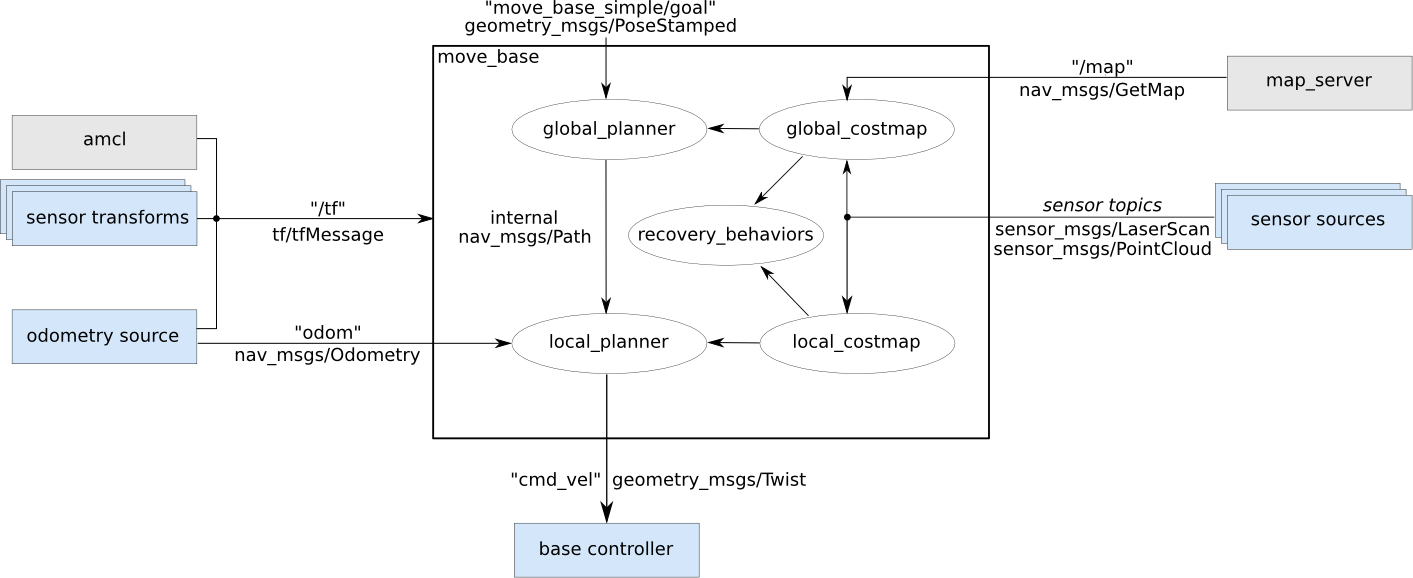
\includegraphics[width=\linewidth]{overview_tf.png}
        \caption{ROS tf stack}
        \label{fig:robot2}
    \end{figure}

    The	navigation stack needs to know the position	of the sensors, wheels, and joints. To do that, we use the	Transform Frames (tf) software library (a huge complex math calculation framework - always good to avoid reinventing the wheel).	

    \section{The robot}
    There are three simulated robots in this work. One build from scratch, a differential simple model, and two models (Innok Heros URDF'S), which are completely modified, practically just the 3D layout and meshes are used. One of them is a skid steering drive, which actually does not work properly with navigation stack, but for the purpose of checking the performance of AMCL, this model was observed too.
    
    \subsubsection{Model design}
    The first robot (scratch-designed) is fairly simple, using standard ROS - URDF files to generate collision, inertia and visuals (CIV). Each element of the robot has its own CIV description. Likes of origin, the xy cordinates where it is mounted to the parent link. Each element is connected to th another thorough a child-parent relation, until to the base-frame. In addition to the basic 3D shapes, there are the more intelegent shapes too, the likes of sensors. Where in addition to the CIV they include the driver code. In our simple robot, those were the wheel joint controller, camera and laser sensor. The drivers (based on ROS C++) publish the ground truth data from the simulator to the respective nodes (refer to the ROS if stack figure above).

    \begin{figure}[!t]
        \begin{tabular}[b]{cc}
          \begin{tabular}[b]{c}
            \begin{subfigure}[b]{0.4\columnwidth}
                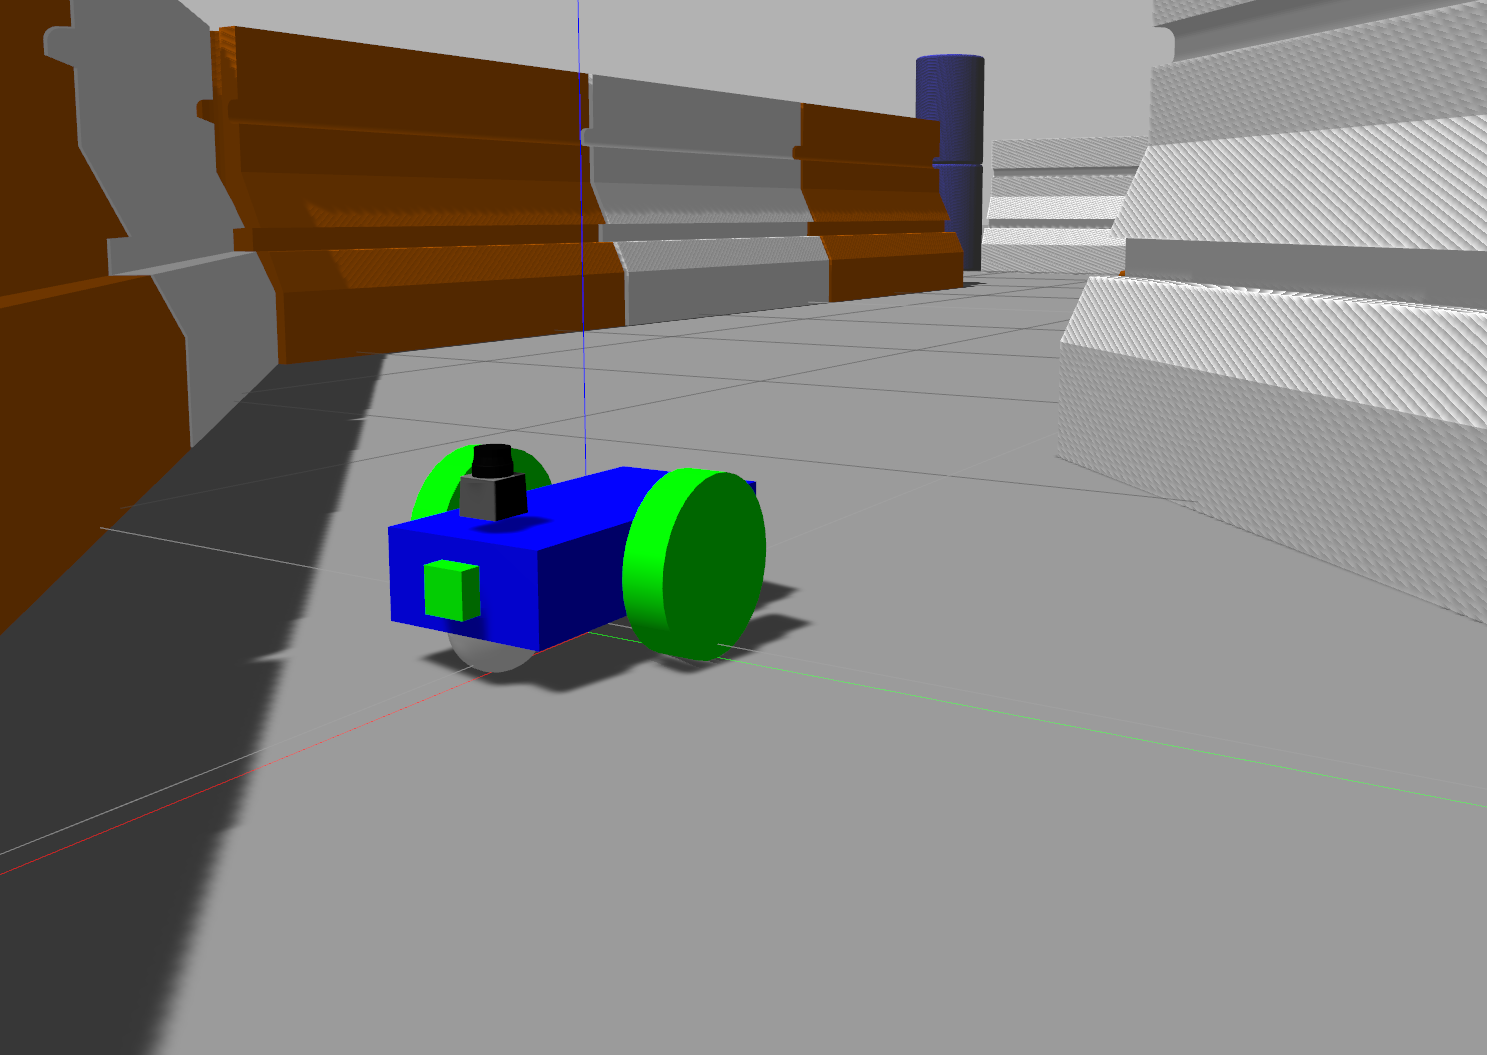
\includegraphics[width=\textwidth]{ubt.png} \caption{ScratchDesigned}
                \label{fig:A} \end{subfigure}\\
            \begin{subfigure}[b]{0.4\columnwidth}
                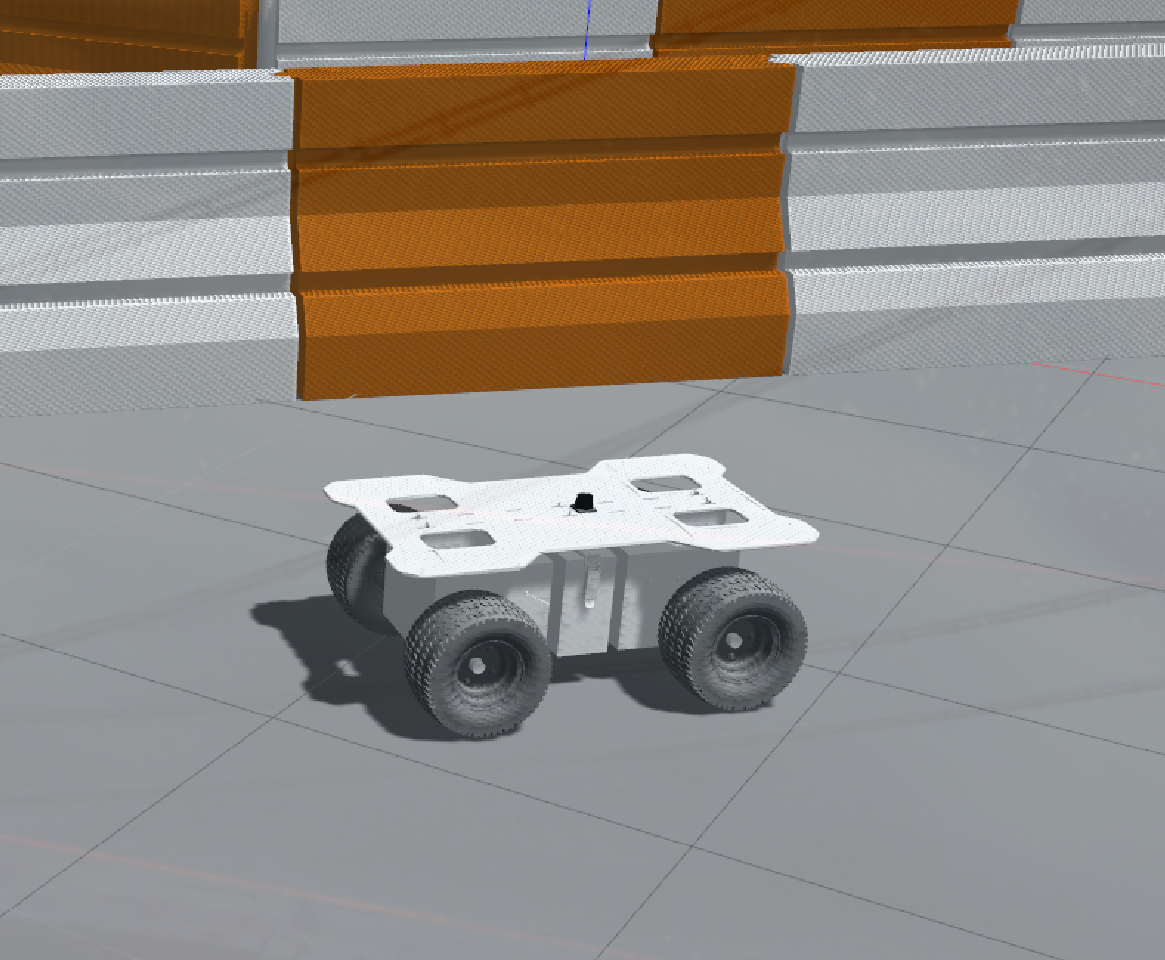
\includegraphics[width=\textwidth]{skid.png} \caption{SkidSteer}
                \label{fig:B} \end{subfigure} \end{tabular}
        & \begin{subfigure}[b]{0.4\columnwidth}
            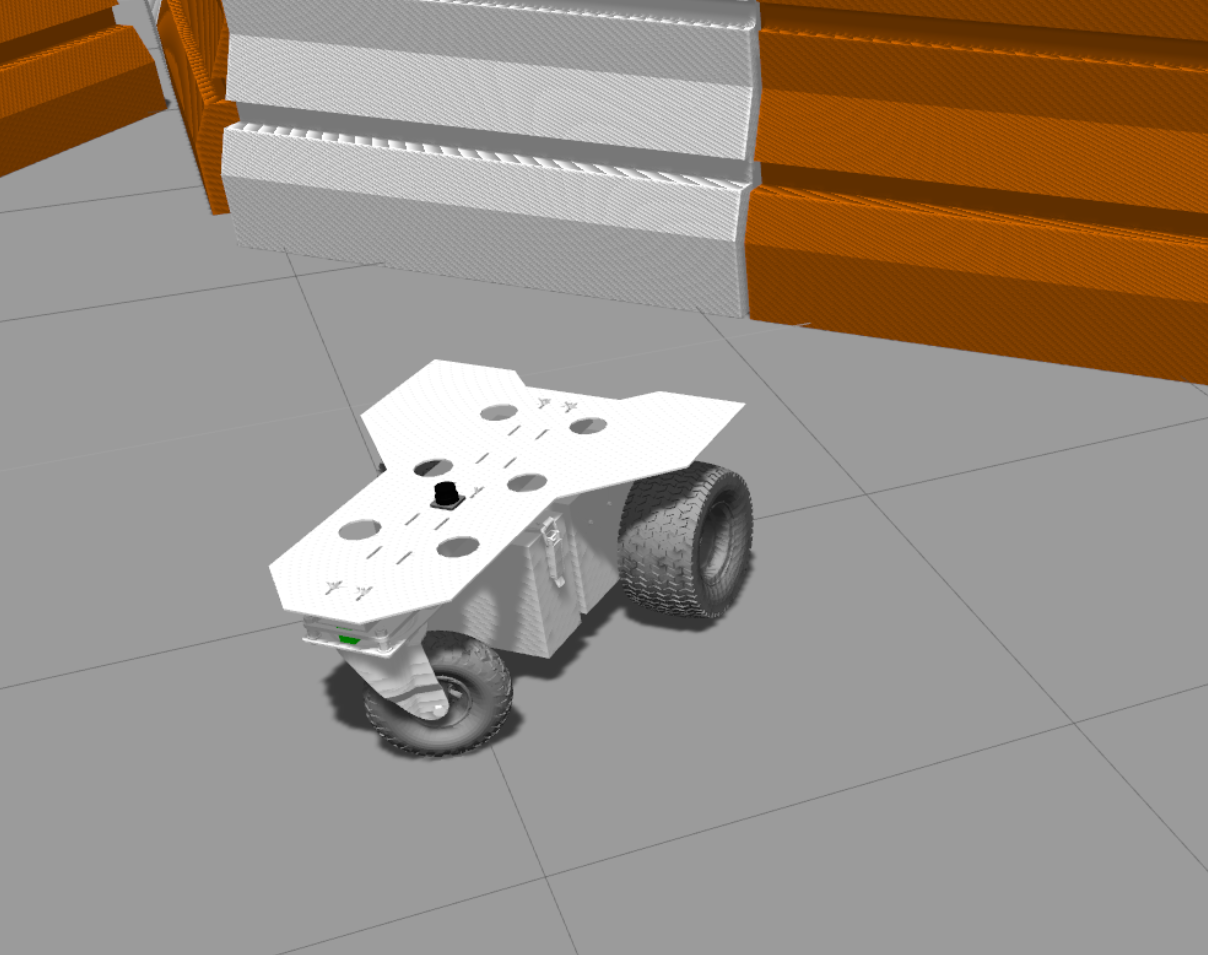
\includegraphics[width=\textwidth]{diss.png} \caption{DiffSteer}
            \label{fig:C} \end{subfigure} \end{tabular} \label{fig:ABC}
            \caption{Different models tested in GAZEBO simulator} \end{figure}

    \subsection{Technical Note} % only facts
    Its worthy mentioning, that since the second model i used was with significant bigger footprint, the position where the robot was spawing was not big enough. So for that i had to make modification in X,Y spawn pose of the robot, and the same time, match this point with AMCL initializing pose.
    
    \subsection{Packages and Parameters}
    As previously mentioned, two base package are used to work in conjunction with each other. MOVE\_BASE and AMCL. For the navigation stack to work as intended (described above), the AMCL algorithm had to be implemented. The AMCL algorithm has many configuration options that will affect the performance of localization. The min\_particles and max\_particles parameters set the minimum and maximum number of particles that are	allowed	for	the	algorithm. With	more particles, you get more accuracy, but this	increases the use of the CPU. The laser\_model\_type parameter is used to configure the laser type. In our	case, we are sing a	 likelihood\_field parameter but the algorithm can also use beam lasers. The laser\_likelihood\_max\_dist parameter is used to set the maximum distance for obstacle inflation on the	map, which is used	in	the	 likelihood\_field model (refer AMCL parameters figure above). 

    In other hand, MOVE\_BASE has its own parameters. It used costmaps to store information about obstacles. One costmap is used for global planning, meaning creating long-term plans over the entire environment, and the other is used for local planning and obstacle avoidance. One of the most important parameters (both for local and global - referred as common costmap) is the laser observation source, which the whole stack defined the obstacles. Its the eyes of the stack. In our case laser scans from scan topic. Another parameter is obstaacle range and raytrace. Those two parameters go hand in had, as the first, based on its valus tells the stack when it sees a obstacle, while the second tell the stack how far is the path free to move on. Another parameter is the robot radius footprint. XY cordinates of each point of frame has to be give, or radius in case of rounded robot. The transform tolerance, represents the time that transform signals are valid for.

    \begin{figure}[thptb]
        \centering
        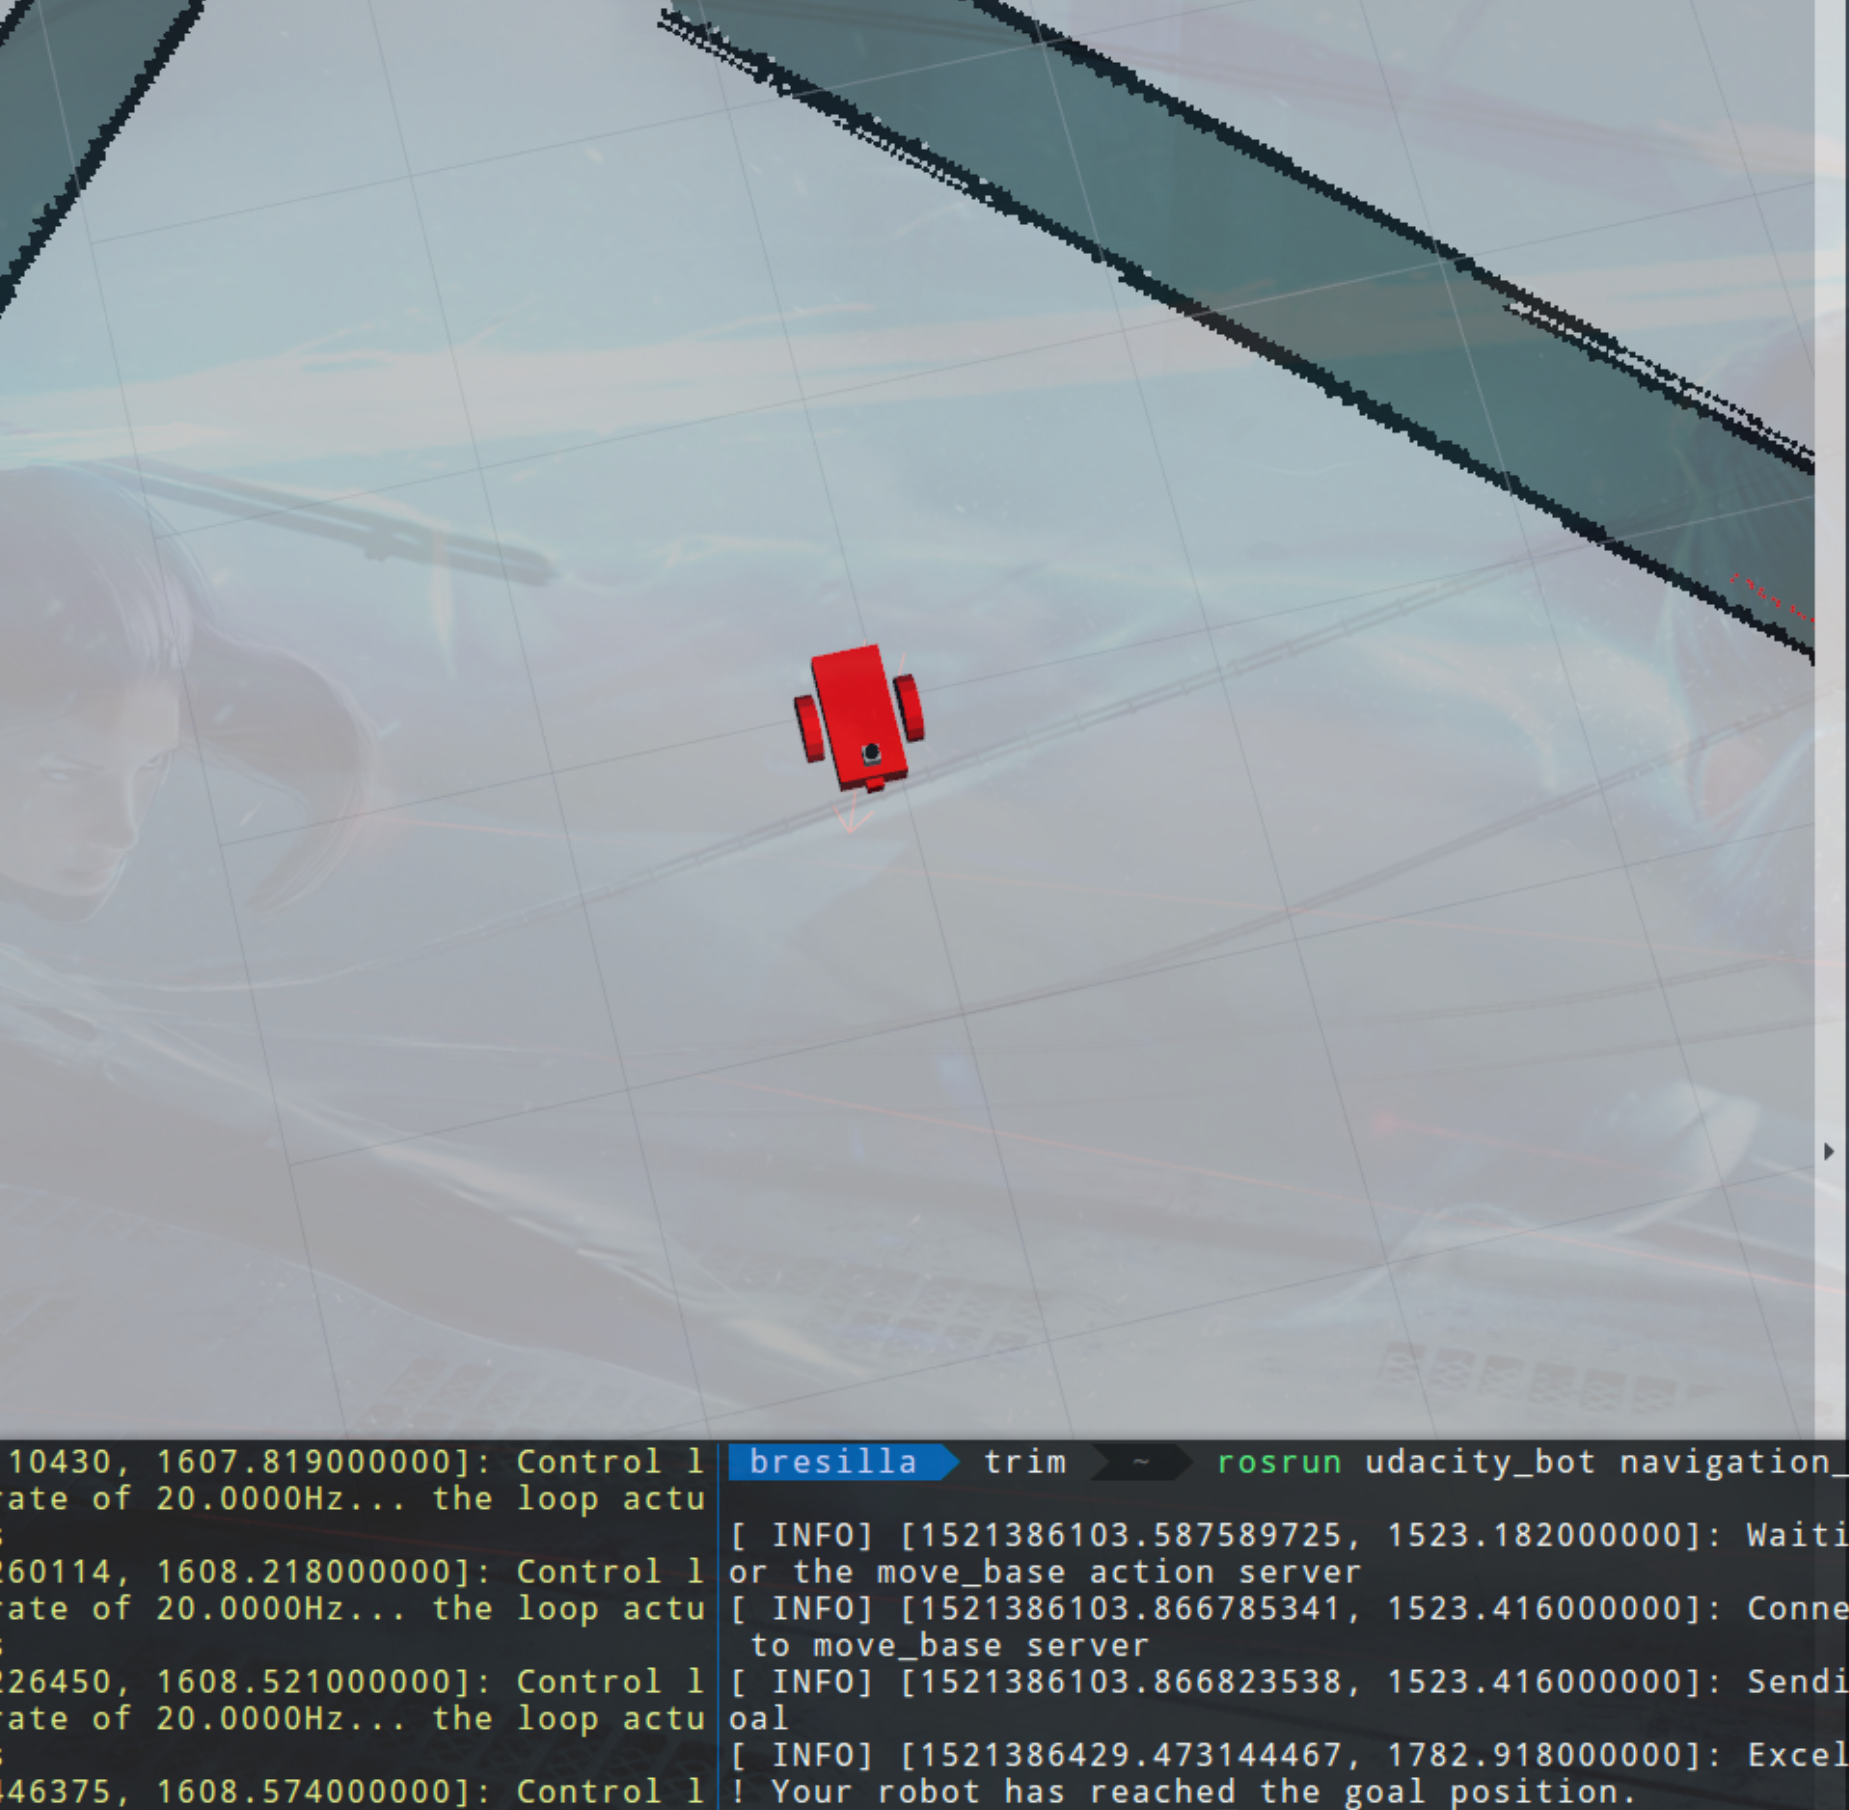
\includegraphics[width=\linewidth]{goal_reched.png}
        \caption{Goal reached}
        \label{fig:robot3}
    \end{figure}
   
     
    \section{Results and Discussion}
    After tweaking (by trial and error) the parameters for AMCL and MOVE\_BASE packages, the robots would perform as expected. The scratched-design bot in a matter of seconds would find its location and would start steering towards the goal (see figure above). While the two other robots, because of their size had difficulties even after countless parameter tweaking, still to locate with precision their pose and perform movement. After spawing them in a different part of the map, where they had more space to manouver (top right part of map), soon they will find the pose and start performing movement.

    As mentioned above, the skid steering drive robot is not properly supported by AMCL package, thus performing not a very optimal drive, but still reaching the target after few minutes.

    The kidnapped scenario, where the robot would spawn in a different location, was very easily solved by AMCL as we used huge amount of particle points, this exacting the pose after just few iterations.
    
    \nocite{*}
    
    \bibliography{bib}
    \bibliographystyle{ieeetr}

    \end{document}